\documentclass[a4paper]{tufte-handout}

\usepackage{algorithm,algorithmic}
\usepackage{graphicx}
\usepackage{framed}
\usepackage{amsmath}
\usepackage[T1]{fontenc}
\usepackage{todonotes}
\usepackage{graphicx}
\hypersetup{
    colorlinks=true,
    linkcolor=blue,
    filecolor=magenta,      
    urlcolor=blue,
}

\title{Deep Learning Training Program}
\author{Sasank Chilamkurthy, Qure.ai}
\date{May 10, 2017}

\begin{document}
\maketitle

\section{Calculus: Recap}\label{calculus-recap}

Let's recap what a derivative is.

\subsection{Derivative}\label{derivative}

Derivative of function \(f(v)\) (\(f'(v)\) or \(\frac{df}{dv}\))
measures sensitivity of change in \(f(v)\) with respect of change in
\(v\).

\begin{figure}
  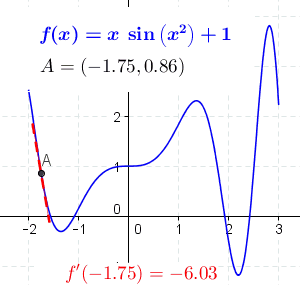
\includegraphics[height=50mm]{differential.png}
  \caption{Derivative illustration. Red is for positive \(v\)
direction and green is for negative \(v\) direction.
\href{https://en.wikipedia.org/wiki/Derivative}{Source}.}
\end{figure}

Direction (i.e sign) of the derivative at a points gives the direction
of (greatest) increment of the function at that point.

\subsection{Gradient}\label{gradient}

The gradient is a multi-variable generalization of the derivative. It is
a vector valued function. For function \(f(v_1, v_2, \ldots, v_n)\),
gradient is a vector whose components are \(n\) partial derivatives of
\(f\):

\[ \nabla f = (\frac{\partial f}{\partial v_1 }, \frac{\partial f}{\partial v_2 }, \ldots, \frac{\partial f}{\partial v_n })\]


\begin{figure}
  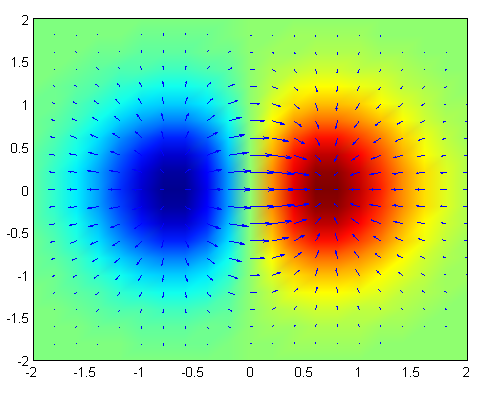
\includegraphics[height=50mm]{gradient.png}
  \caption{Gradient of the 2D function \(f(x, y) = xe^{−(x^2 + y^2)}\) is
plotted as blue arrows over the pseudocolor (red is for high values
while blue is for low values) plot of the function.
\href{https://en.wikipedia.org/wiki/Gradient}{Source}.}
\end{figure}


Similar to derivative, direction of the gradient at a point is the
steepest ascent of the function starting from that point.

\section{Optimization}\label{optimization}

Given a function \(C(v_1, v_2, \ldots, v_n)\), how do we optimize it?
i.e, find a point which minimizes this function globally.

This is a very generic problem; lot of practical and theoretical
problems can be posed in this form. So, there is no general answer.

\subsection{Gradient Descent}\label{gradient-descent}

However, for a class of functions called convex functions, there is a
simple algorithm which is guaranteed to converge to minima. Convex
functions have only one minima. They look something like this:

\begin{figure}
  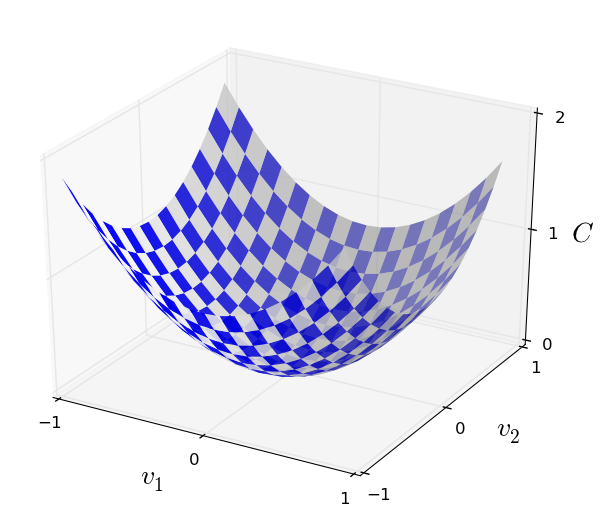
\includegraphics[width=100mm]{valley.png}
  \caption{A 2d convex function. 
  			\href{http://neuralnetworksanddeeplearning.com/chap1.html}{Source}.}
\end{figure}


To motivate our algorithm, imagine this function as a valley and a ball
is put at a random point on the valley and allowed to roll. Our common
sense tells that ball will eventually roll to the bottom of the valley.

\begin{figure}
  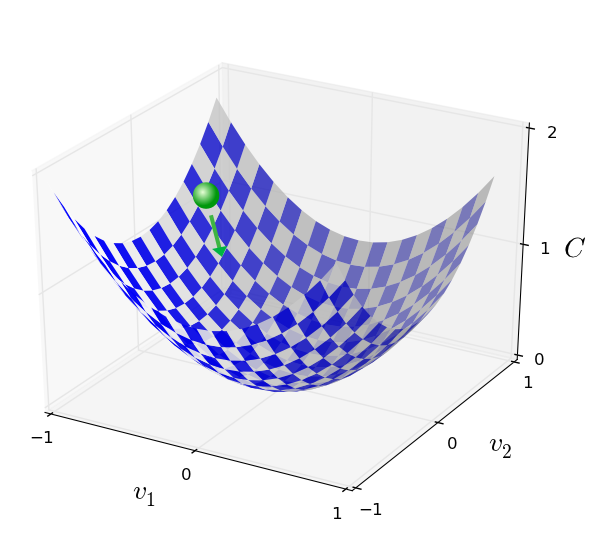
\includegraphics[width=50mm]{valley_with_ball}
  \caption{Gradient descent illustration: a ball on a valley.
\href{http://neuralnetworksanddeeplearning.com/chap1.html}{Source}.}
\end{figure}

Let's roughly simulate the motion of the ball! Key observation is that
the ball moves in the steepest direction of descent. This is negative
\sidenote{Gradient gives us steepest direction of \emph{ascent}.}
of the gradient's direction.

Great! Let's put together our algorithm:

\begin{algorithm}
\caption{Gradient Descent}
\begin{algorithmic}[1]
  \STATE Start at a random point: \(v\)
  \WHILE{\(v\) doesn't converge}
  \STATE Update \(v\) in the direction of steepest descent: 
      \[v \rightarrow v' = v -\eta \nabla C\]
  \ENDWHILE
\end{algorithmic}
\end{algorithm}

\begin{marginfigure}[-40mm]
  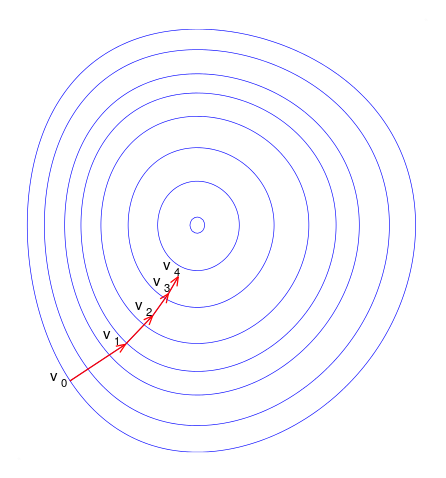
\includegraphics[width=50mm]{Gradient_descent}
  \caption{Gradient descent on a series of level sets.
  \href{https://en.wikipedia.org/wiki/Gradient_descent}{Source}.}
\end{marginfigure}


Here \(\eta\) is called \emph{learning rate}. If it is too small,
algorithm can be very slow and might take too many iterations to
converge. If it is too large, algorithm might not even converge.

\subsection{Example: Regression}\label{example-regression}

Let's apply the things learnt above on linear regression problem. Here's
a recap of linear regression:

\begin{quote}
Our model is \(y(x) = wx + b\). Parameters are \(v = (w, b)\) We are
given training pairs \((x^1, y^1), (x^2, y^2), \ldots, (x^n, y^n)\)
\sidenote{ Notation clarifiction: Here, superscripts are indices, not powers }.

We want to find \(w\) and \(b\) which minimize the following cost/loss
function:

\[ C(w, b) = \frac{1}{n} \sum_{i = 1}^{n} C_i(w, b) = \frac{1}{2n} \sum_{i = 1}^{n} \| y(x^i) - y^i\|^2 \]

where
\(C_i(w, b) = \frac{1}{2} \| y(x^i) - y^i\|^2 = \frac{1}{2} \| wx^i + b - y^i\|^2\)
is the loss of the model for \(i\) th training pair.
\end{quote}


Let's calculate gradients,

\[ \nabla C = \frac{1}{n} \sum_{i = 1}^{n} \nabla C_i \]

where \(\nabla C_i\) is computed using:

\[ \nabla C_i = \left( \frac{\partial C_i}{\partial w}, \frac{\partial C_i}{\partial b}  \right) = \left( (wx^i + b - y^i)x^i, (wx^i + b - y^i) \right)\]

Update rule is

\[ v \rightarrow v' = v -\eta \nabla C = v -\frac{\eta}{n} \sum_{i = 1}^{n} \nabla C_i \]


\subsection{Stochastic Gradient Descent}\label{stochastic-gradient-descent}

In the above example, what if we have very large number of samples i.e
\(n \gg 0\)? At every optimization step, we have to compute
\(\nabla C_i\) for each sample \(i = 1, 2, \ldots, n\). This can be very
time consuming!

Can we approximate \(\nabla C\) with a very few samples? Yes!

\[ \nabla C = \frac{1}{n} \sum_{i = 1}^{n} \nabla C_i \approx \frac{1}{m} \sum_{j \in S_m} \nabla C_j \]

where \(S_m\) is random subset of size \(m \ll n\) of
\({1, 2, \ldots,n}\). It turns out that this approximation, even though
estimated only from a small random subset of samples, is good enough for
convergence of gradient descent. This subset of data is called
\emph{minibatch} and this technique is called \emph{stochastic gradient
descent}.

Then stochastic gradient descent works by picking a randomly chosen
subset of data and trains (i.e updates \(v\)) with gradient
approximation computed from them. Next, another subset is picked up and
trained with them. And so on, until we've exhausted all the training
data, which is said to complete an \emph{epoch} of training. Concretely,
following is the stochastic gradient descent algorithm.

\begin{algorithm}
\caption{Stochastic Gradient Descent}
\begin{algorithmic}[1]
  \STATE Start at a random point: \(v\)
  \FOR{a fixed number of epochs}
      \STATE Randomly partition the data into minibatches each of size $m$ 
      \FOR{For each minibatch $S_m$}
        \STATE Update the parameters using \[v \rightarrow v' = v -\frac{\eta}{m} \sum_{i \in S_m} \nabla C_j\]
      \ENDFOR
  \ENDFOR
\end{algorithmic}
\end{algorithm}

\section{Neural Networks}\label{neural-networks}

With this background, we are ready to start with neural networks.

\subsection{Perceptron}\label{perceptron}

Perceptron, a type of artificial neuron was developed in the 1950s and
1960s. Today, it's more common to use Rectified Linear Units (ReLUs).
Nevertheless, it's worth taking time to understand the older models.

So how do perceptrons work? A perceptron takes several inputs,
\(x_1, x_2, \ldots x_n\) and produces a single output:


\begin{figure}
  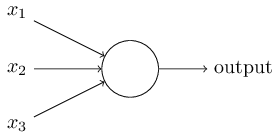
\includegraphics[width=60mm]{tikz0}
  \caption{ Perceptron Model.
\href{http://neuralnetworksanddeeplearning.com/chap1.html}{Source}. }
\end{figure}


\emph{Weights} \(w_1, w_2, \ldots w_n\) decide the importance of each of
the inputs on output \(y(x)\). There is also a \emph{threshold} \(b\) to
decide the output. These are the parameters of the model.

The expression of the output is

\[ y(x) = \sigma\left(\sum_j w_j x_j - b\right) \]

where \(\sigma(z)\) is step function, 

\begin{eqnarray*}
  \sigma(z) & = & \left\{ \begin{array}{ll}
      0 & \mbox{if } z \leq 0 \\
      1 & \mbox{if } z > 0
      \end{array} \right.
\end{eqnarray*}

Therefore 
\begin{eqnarray*}
    y(x) & = & \left\{ \begin{array}{ll}
      0 & \mbox{if } \sum_j w_j x_j \leq b \\
      1 & \mbox{if } \sum_j w_j x_j > b
      \end{array} \right.
\end{eqnarray*}

That's the basic mathematical model. A way you can think about the
perceptron is that it's a device that makes decisions by weighing up
evidence. An example
\sidenote{This example is straight from
\href{http://neuralnetworksanddeeplearning.com/chap1.html}{here}}:

Another way perceptrons can be used is to compute the elementary logical
functions we usually think of as underlying computation, functions such
as \texttt{AND}, \texttt{OR}, and \texttt{NAND}. Check that following
perceptron implements \texttt{NAND}:

\begin{figure}
  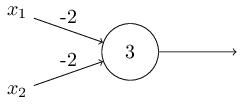
\includegraphics[width=60mm]{tikz2}
  \caption{\texttt{NAND} implemented by perceptron.
\href{http://neuralnetworksanddeeplearning.com/chap1.html}{Source} }
\end{figure}

If you are familiar with digital logic, you will know that \texttt{NAND}
gate is a universal gate. That is, any logical computation can be
computed using just \texttt{NAND} gates. Then, the same property follows
for perceptrons.

\subsection{Multi Layer Perceptrons and Sigmoid}
\label{multi-layer-perceptrons-and-sigmoid}

Although perceptron isn't a complete model of human decision-making, the
above example illustrates how a perceptron can weigh up different kinds
of evidence in order to make decisions. And it should seem plausible
that a complex network of perceptrons could make quite subtle decisions

\begin{figure}
  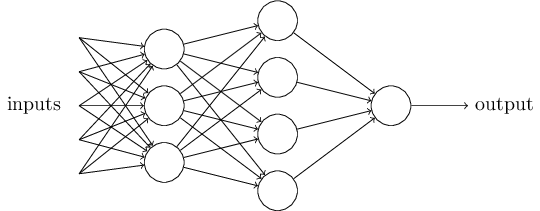
\includegraphics[height=35mm]{tikz1}
  \caption{Multi layer perceptron.
\href{http://neuralnetworksanddeeplearning.com/chap1.html}{Source} }
\end{figure}

This network is called \emph{Multi layered perceptron (MLP)}. In this
MLP, the first column of perceptrons - what we'll call the first
\emph{layer} of perceptrons - is making three very simple decisions, by
weighing the input evidence. What about the perceptrons in the second
layer? Each of those perceptrons is making a decision by weighing up the
results from the first layer of decision-making. In this way a
perceptron in the second layer can make a decision at a more complex and
more abstract level than perceptrons in the first layer. And even more
complex decisions can be made by the perceptron in the third layer. In
this way, a many-layer network of perceptrons can engage in
sophisticated decision making.

How do we learn the parameters of the above model? Gradient Descent!
\sidenote{ MLP model is far from convex.
Therefore, gradient descent is not guaranteed to converge! But it turns
out that it works fine with a few tweaks which we describe below.}
However, the network is very discontinuous. In fact, a small change in
the weights or bias of any single perceptron in the network can
sometimes cause the output of that perceptron to completely flip, say
from 0 to 1. This makes it very difficult for gradient descent to
converge.

How do we overcome this? What is the source of this discontinuity?
Remember that output of perceptron is given by
\(y(x) = \sigma\left(\sum_j w_j x_j - b\right)\) where \(\sigma(z)\) is
step function

\begin{eqnarray*}
  \sigma(z) & = & \left\{ \begin{array}{ll}
      0 & \mbox{if } z \leq 0 \\
      1 & \mbox{if } z > 0
      \end{array} \right.
\end{eqnarray*}

This \(\sigma(z)\) is the source of discontinuity. Can we replace
step function with a smoother version of it?

Check out the following function:

\begin{eqnarray*} 
  \sigma(z) = \frac{1}{1+e^{-z}}.
\end{eqnarray*}

If you graph it, it's quite clear that this function is smoothed out
version of a step function. This function is called \emph{sigmoid}.

\begin{figure}
  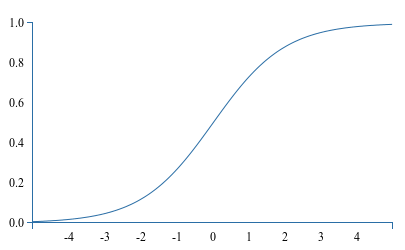
\includegraphics[height=45mm]{sigmoid}
  \caption{Sigmoid function. When \(z\) is large and
  positive, Then \(e^{-z} \approx 0\) and so \(\sigma(z) \approx 1\).
  Suppose on the other hand that \(z\) is very negative. Then
  \(e^{-z} \rightarrow \infty\), and \(\sigma(z) \approx 0\).
  \href{http://neuralnetworksanddeeplearning.com/chap1.html}{Source}.}
\end{figure}

With the \emph{sigmoid neuron}, gradient descent usually converges.
Before computing gradients for gradient descent, we need to discuss loss
functions\sidenote{I use terms loss function and
cost function interchangeably.} and activation functions.


\subsection{Activation and Loss
Functions}\label{activation-and-loss-functions}

By now, you have seen that general form of a artificial neuron is
\(y(x) = \sigma\left( w^T x + b\right)\).
\protect\hypertarget{activation}{}{} { I have rewritten sum
\(\sum_j w_j x_j\) as dot product \(w^Tx\) and changed the sign of
\(b\). }. Here the function \(\sigma(z)\) is called \emph{activation
function}. So far, we have seen two different activations:

\begin{enumerate}
\item
  Step function
\item
  Sigmoid function
\end{enumerate}

\noindent \emph{ReLU}:

Let me introduce another activation function, \emph{rectifier} or
\emph{rectified linear unit} (ReLU):

\[\sigma(z) = \max(0, z)\]

Its graph looks like this: 

\begin{figure}
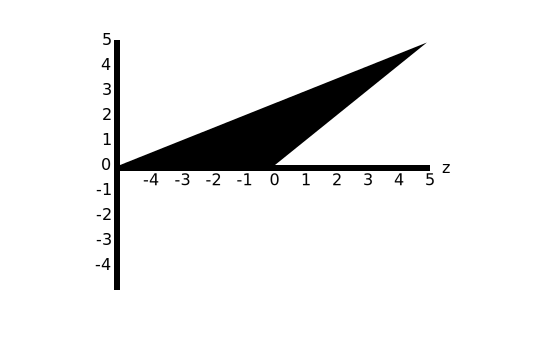
\includegraphics[height=55mm]{relu}
\caption{ ReLU.
\href{http://neuralnetworksanddeeplearning.com/chap3.html}{Source}. }
\end{figure}

Because of technical reasons 
\sidenote{ More
specifically, because of vanishing and exploding gradients problem. Read
more \href{http://neuralnetworksanddeeplearning.com/chap5.html}{here}},
ReLUs are preferred activation functions these days. You will almost
never see sigmoid activation function in modern deep neural networks.

\hfill

\noindent \emph{Loss functions:}

Let's discuss loss/cost functions now. We will make two assumptions
about our cost function:

\begin{enumerate}
\item
  The cost function can be written as an average over cost functions
  \(C_i\) for individual training examples, \((x^i, y^i)\). i.e,
  \(C = \frac{1}{n} \sum_{i = 1}^{n} C_i\)
\item
  Cost can be written as a function of the outputs from the neural
  network. i.e, \(C_i = L(y(x^i), y^i)\) where \(y(x)\) is the output
  from the network.
\end{enumerate}

In the case of regression, we used \(L_2\) loss,
\(L(o, y) = \frac{1}{2} \| o - y\|^2\). We could have also used \(L_1\)
loss, \(L(o, y) = \| o - y \|_{L_1}\).

\hfill

\noindent \emph{Cross Entropy Loss:}

What if we have a classification problem? What loss do we use? Consider
the following MLP for digit classification:

\begin{figure}
  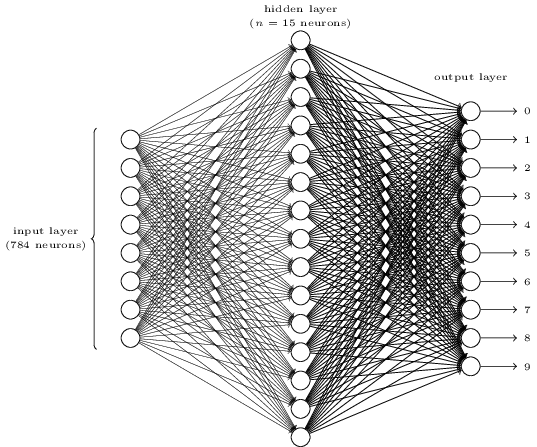
\includegraphics[height=80mm]{tikz12}
  \caption{ MLP for digit classification.
  \href{http://neuralnetworksanddeeplearning.com/chap1.html\%22}{Source}.
  }
\end{figure}

Here, we have output \(o\) of size 10 and a target class \(y\). We could
have used \(L_1(o, e_y)\) or \(L_2(o, e_y)\) loss where \(e_y\) is
\(y\)th unit vector. But it turns out that this doesn't work very well.

Instead, We will consider the outputs as a probability distribution over
10 classes and use what is called a cross entropy loss:

\[ L(o, y) = - \log(o_y) \]

To understand this function, realize that \(o_y\) is the output
probability of the target class \(y\). Minimizing negative of log of
this probability, maximizes the probability. Also, \(L \geq 0\) because
\(\log(x) < 0\) for \(x \in [0, 1]\).

\hfill

\noindent \emph{Softmax Activation:}

If we use cross entropy loss, we cannot use sigmoids as activations of
output layer because sigmoids do not guarantee a probability
distribution. Although each component of the output is in \([0, 1]\),
they need not add up to 1.

We therefore use an activation layer called \emph{softmax}. According to
this function, the activation \(a_j\) of the \(j\)th output neuron is

\[ a_j = \frac{e^{z_j}}{\sum_k e^{z_k}} \]

where in the denominator we sum over all the output neurons.
This expression may seem opaque if you are not familiar with it. Observe
the following:

\begin{enumerate}
\item
  Activations are positive: \(a_j \geq 0\)
\item
  Activations sum to 1: \(\sum_j a_j = 1\)
\item
  If you increase \(z_m\) keeping others constant, \(a_m\) increases.
  Other activations decrease to ensure sum remains 1.
\item
  If \(z_m\) is much larger than the others, \(a_m \approx 1\) and
  \(a_k \approx 0\) for \(k \neq m\).
\end{enumerate}

Therefore softmax is a probability distribution which behaves like
smooth version of \texttt{argmax}.

\subsection{Backpropogation}\label{backpropogation}

We have so far discussed the model component of neural networks. We
haven't yet discussed how we learn the parameters of the networks.

As expected, we will use stochastic gradient descent. For this, we need
gradients of \(C_i\), loss for the \(i\)th training example. Computation
of this quantity, \(\nabla C_i\) is slightly involved. Let's start with
writing the expression for \(C_i\). Let's represent all the parameters
of the network with \(\theta\):

\[ C_i(\theta) = L\left(y(x^i, \theta), y^i \right)\]

Let's break the above function into composition of functions (or
layers).

\[ C = y_n \circ \ y_{n-1} \circ \cdots \circ y_1 \]

Here, \(i\)th \sidenote{ In particular,
\(C = o_n = y_n(u_n) = L(u_n, x_i)\) } function takes in input \(u_i\)
and outputs

\begin{equation}
o_i = y_i(u_i, \theta_i) \label{eq:1}
\end{equation}


where \(\theta_i\) are learnable parameters of this function. Since
output of \(i-1\)th layer is fed to \(i\)th layer as input,

\begin{equation}
u_i = o_{i-1} \label{eq:2}
\end{equation}


We require
\(\nabla C = \left(\frac{\partial C}{\partial\theta_1}, \frac{\partial C}{\partial\theta_2}, \ldots, \frac{\partial C}{\partial\theta_n}\right)\).
Therefore, we need to compute, for  \( j = 1, 2, \dots n \)

\[ \frac{\partial C}{\partial\theta_j} = \frac{\partial o_n}{\partial\theta_j} \]

To compute this quantity, we will compute generic
\sidenote{ You will see ahead why this quantity is useful. }:

\[ \frac{\partial o_i}{\partial \theta_j} \]

Before getting started, let's write down the chain rule. Chain rule is
the underlying operation of our algorithm.

\begin{framed}
For function f(x, y), 

\begin{equation}
\frac{\partial f}{\partial t} = \frac{\partial f}{\partial x} * \frac{\partial x}{\partial t} + \frac{\partial f}{\partial y} * \frac{\partial y}{\partial t}
\label{eq:3}
\end{equation}

\end{framed}

If \(j > i\),

\begin{equation}
\frac{\partial o_i}{\partial \theta_j} = 0 \label{eq:4}
\end{equation}


because output of the functions in back doesn't depend on parameters of
layer in the front.

If \(j = i\), using equation \eqref{eq:1} and the fact that \(u_i\) and
\(\theta_i\) are independent,

\begin{equation}
\frac{\partial o_i}{\partial \theta_i} = \frac{\partial y_i}{\partial \theta_i}
 \label{eq:5}
\end{equation}

\(\frac{\partial y_i}{\partial \theta_i}\) is a computable quantity
which depends on the form of function \(y_i\).

If \(j < i\), using equation \eqref{eq:1}, \eqref{eq:2}, chain rule \eqref{eq:3},

\begin{align*}
\frac{\partial o_i}{\partial \theta_j} &= \frac{\partial y_i}{\partial \theta_j}\\
&= \frac{\partial y_i}{\partial u_i} * \frac{\partial u_i}{\partial \theta_j} + \frac{\partial y_i}{\partial \theta_i} * \frac{\partial \theta_i}{\partial \theta_j}\\
&= \frac{\partial y_i}{\partial u_i} * \frac{\partial u_i}{\partial \theta_j}\\
&= \frac{\partial y_i}{\partial u_i} * \frac{\partial o_{i-1}}{\partial \theta_j}
\end{align*}


Therefore,

\begin{equation}
\frac{\partial o_i}{\partial \theta_j} = \frac{\partial y_i}{\partial u_i} * \frac{\partial o_{i-1}}{\partial \theta_j}
\label{eq:6}
\end{equation}

Like \(\frac{\partial y_i}{\partial \theta_i}\),
\(\frac{\partial y_i}{\partial u_i}\) is a computable quantity which
depends on \(y_i\).

\noindent Let's put everything together and compute the required quantity
\sidenote{Apply \eqref{eq:6} repetitively}:

\begin{align*}
\frac{\partial C}{\partial \theta_j} &= \frac{\partial o_n}{\partial \theta_j}\\
&= \frac{\partial y_n}{\partial u_n} * \frac{\partial o_{n-1}}{\partial \theta_j}\\
&= \frac{\partial y_n}{\partial u_n} * \frac{\partial y_{n-1}}{\partial u_{n-1}} * \frac{\partial o_{n-2}}{\partial \theta_j} \\
&\vdots \\
&= \frac{\partial y_n}{\partial u_n} * \frac{\partial y_{n-1}}{\partial u_{n-1}} * \cdots * \frac{\partial y_{j-1}}{\partial u_{j-1}} * \frac{\partial o_j}{\partial \theta_j}\\
&= \frac{\partial y_n}{\partial u_n} * \frac{\partial y_{n-1}}{\partial u_{n-1}} * \cdots * \frac{\partial y_{j-1}}{\partial u_{j-1}} * \frac{\partial y_j}{\partial \theta_j}
\end{align*}

Now, algorithm to compute gradients \(\nabla C\), i.e.
\(\frac{\partial C}{\partial \theta_j}\) for all \(j\) is fairly clear.

\begin{algorithm}[H]
\caption{Back Propogation}
\begin{algorithmic}[1]
  \STATE \{Forward pass\}
  \STATE Set \(u_0 = x\)
  \FOR {\(i = 1, \dots n\)}
  	\STATE Store \(u_i = y_i(u_{i-1}, \theta_i)\)
  \ENDFOR
  \STATE \{Backward pass\}
  \STATE {Set \(\texttt{buffer} = 1\)}
  \FOR {\(j = n, n-1, \dots 1\)}
  	\STATE Store \(\frac{\partial C}{\partial \theta_j} = \frac{\partial y_j}{\partial \theta_j} * \texttt{buffer}\)
  	\STATE Update \(\texttt{buffer} = \frac{\partial y_j}{\partial u_j} * \texttt{buffer}\)
  \ENDFOR 
  \RETURN \(\left(\frac{\partial C}{\partial\theta_1}, \frac{\partial C}{\partial\theta_2}, \ldots, \frac{\partial C}{\partial\theta_n}\right)\).
\end{algorithmic}
\end{algorithm}


Although this derivation is for scalar functions, it will work with
vector functions with a few modifications.

\section{Deep Networks}
\end{document}